% !TEX root = QlockToo.tex
% Kapitelvorlage
\begin{multicols}{2}
\section{Elektronik}
\label{sec:Elektronik}
Die LED-Matrix mit 10 x 11 Pixel wird von einem Mikrocontroller angesteuert, dies geschieht zeilenweise im Multiplexing-Verfahren. Hierbei wird eine der 10  Zeilen von einem Transistor mit Spannung versorgt und die 11 Pixel der Zeile über einen LED-Treiber simultan angesteuert. Nach einer Millisekunde wird die Zeile ausgeschaltet, neue Daten in den LED-Treiber geschrieben und die nächste Zeile eingeschaltet. 
\subsection{Arduino Micro}
Als Mikrocontroller wird ein Arduino Micro Board mit dem Atmel Atmega 32U4 Controller verwendet. Der Einsatz eines Arduino Boards vereinfacht die Umsetzung einer seriellen Schnittstelle und verringert durch das bereits vielfach genutzte Board die Fehlerquellen im Layout. Durch die kleine Bauform und die sich aus den Features ergebenden Anforderungen (serielle Kommunikation, $I^{2}C$-Bus, externer Interrupt, 4x Digital Input 2x Analogeingang und 10x Digital Output) fiel die Auswahl auf den Arduino Micro.

\begin{figure}[h]
    \centering
    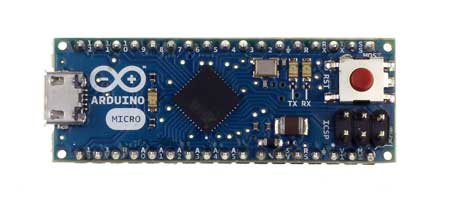
\includegraphics[width=\columnwidth]{Abbildungen/ArduinoMicro}
    \caption[Arduino Micro]{Der Arduino Micro}
    \label{fig:ArduinoMicro}
\end{figure}

\subsection{LED-Treiber}
Der TLC59116 LED-Treiber von Texas Instruments hat 16 PWM-Ausgänge mit 8Bit Auflösung - 255 Helligkeitsstufen - und eine Stromregelung, die es ermöglicht auf Vorwiderstände an den LED zu verzichten. Der IC wird über $I^{2}C$ angesteuert.Die Adresse kann hardwareseitig in den letzten 4Bit eingestellt werden und ist auf der Platine hart mit 0b1100 000[R/W] adressiert. Der LED-Treiber ist in der SMD TSSOP-28 Bauform.
\subsection{Transistoren}
Die Zeilen werden mit IRF7416 P-FET-Transistoren geschaltet und mit $5V$ versorgt. Die Transistoren werden mit einem Pull-Up Widerstand am Gate beschaltet und mit einem invertierten Signal angesteuert (4 - 13). Die Transistoren haben S0-8 Gehäusebauform. 
\subsection{Taster}
Die vier Kurzhubtaster an der rechten Rahmenseite befinden sich auf einer eigenen Platine mit Verbindungskabel. Zur Entprellung befindet sich kurz vor den vier IO-Pins (A2 - A5) des Controllers ein RC-Glied. 
\subsection{Sensoren}
Als Helligkeitssensor wird ein LDR und als Temperatursensor ein NTC verwendet. In beiden Fällen mit einem Trimmpoti als Spannungsteiler an einem Analogeingang (A0 - A1) des Mikrocontrollers.
\subsection{DCF 77}
Das DCF77-Modul empfängt das Mitteleuropäische Zeitsignal und verstärkt es. Um das Signal problemlos zu Empfangen wird hier ein interruptfähiger Eingang des Mikrocontrollers (1) verwendet. Durch regelmäßigen Empfang des DCF77 Zeitsignals ist die Genauigkeit des verbauten Quarz hinreichend genau.

\end{multicols}